\section{Tasks and Schedule}
The main tasks of which the \textit{PowerEnJoy} project is composed of are the following:
\begin{enumerate}
\item \textbf{Requirements Analysis and Specification Document (RASD)} delivery - deliver a document containing the description of all goals, domain assumptions, functional and non-functional requirements for the project;
\item \textbf{Design Document (DD)} delivery - deliver a document describing the architectural design of the software system to be produced;
\item \textbf{Integration Test Plan Document (ITPD)} delivery - deliver a document containing the strategy to perform integration testing on the components of the system;
\item \textbf{Project Plan Document (PPD)} delivery - deliver a document containing the description of the schedule and tasks for the project and an estimation of the effort and size of the project itself, as well as an analysis of the risks that the project could face during its life-cycle;
\item \textbf{Implementation} - implement the software product and thoroughly write unit tests for all the code;
\item \textbf{Integration testing} - test the integration of all the software components of the project;
\end{enumerate}

During the project life-cycle, some of these task can not begin if others are not completed yet. To illustrate the precedence constraints of the case, a \textbf{dependency graph} is provided in Figure \ref{dep_dag}.

Note that, however, since a software project is highly subject to change in requirements and evolves continuously, there might be the need of coming back to previous tasks one or more times after the conclusion of said tasks themselves.

\begin{figure}[H]
\begin{center}
		\centerline{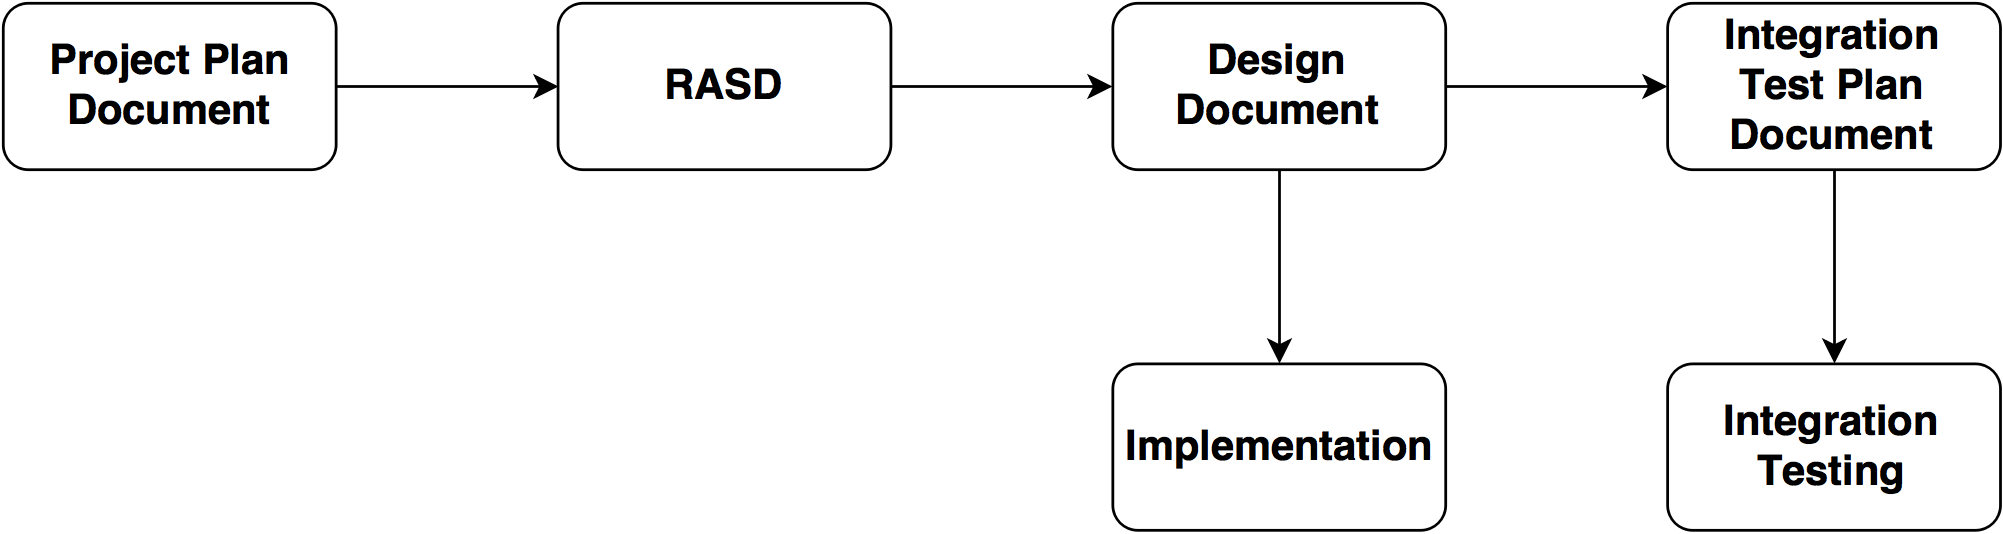
\includegraphics[width=\textwidth]{./pictures/dependencies_dag.png}}
		\caption{Dependency graph illustrating precedence constraints.}
		\label{dep_dag}
\end{center}
\end{figure}
\noindent
The following is a Gantt chart to describe the chosen schedule for the project:

%gantt chart here

\section{Resource Allocation}
Given the tasks defined above, the allocation of human resources of the team to the single tasks and their sub-parts is going to be defined in this section. Since the team is only composed of two members, the granularity of the activities composing the tasks is quite rough: this is to avoid a pointless level of detail in favour of an easier-to-understand allocation of macro-activities.

Note that most activities involve contribution from both team members, either in a parallel fashion or in a cooperative way. This is done in order to increase the awareness of the team with respect to the single tasks of the project, so that all the members can be work on any part of the system in case of necessity, without spending too much time understanding it; this also reduces the risk of misunderstandings between team members and increases the efficiency of cooperative work sessions.

The following tables describe in detail the subdivision of every task in different activities, as well as the allocation of team members to the single activities themselves. The duration of tasks and activities is structured based on the considerations and conclusions expressed in the sections above.

Activities on the same row represent activities executed in parallel. If the same activity is marked twice on the same row, that activity is executed in cooperation by both team members.

\begin{table}[H]
	\begin{adjustwidth}{-.5in}{-.5in}
    \centering
    \begin{tabular}{ p{0.12\textwidth} | p{0.45\textwidth} | p{0.45\textwidth} }
    	\hline
    	& \multicolumn{1}{c |}{\textbf{Giovanni}} & \multicolumn{1}{c}{\textbf{Marco}} \\
    	\hline
		\hline
        \multirow{4}{*}{\textbf{$1_{st}$ week}}
        & Risk Management & Introduction \\ \cline{2-3}
        & FPs Estimation & FPs Estimation \\ \cline{2-3}
        & COCOMO II Effort Estimation & COCOMO II Effort Estimation \\ \cline{2-3}
        & Resource Allocation & Resource Allocation \\ \cline{2-3}
        & Review Resource Allocation & Review Risk Management \\
        \hline
    \end{tabular}
    \caption{Resource allocation for Project Plan Document.}
    \label{ppd_allocation}
    \end{adjustwidth}
\end{table}

\begin{table}[H]
    \begin{adjustwidth}{-.5in}{-.5in}
    \centering
    \begin{tabular}{ p{0.12\textwidth} | p{0.45\textwidth} | p{0.45\textwidth} }
    	\hline
    	& \multicolumn{1}{c |}{\textbf{Giovanni}} & \multicolumn{1}{c}{\textbf{Marco}} \\
    	\hline
		\hline
        \multirow{4}{*}{\textbf{$1_{st}$ week}} & Purpose, Scope & References, Overview \\ \cline{2-3}
        & Initial goals draft & Initial goal draft \\ \cline{2-3}
        & Product Perspective & Product Functions, Constraints \\ \cline{2-3}
        & User Characteristics & Constraints \\ \cline{2-3}
        \hline
        \hline
         \multirow{2}{*}{\textbf{$2_{nd}$ week}} & Initial assumptions draft & Initial assumptions draft \\ \cline{2-3}
        & Goals & Assumptions and Dependencies \\
        \hline
        \hline
        \multirow{4}{*}{\textbf{$3_{rd}$ week}} & Initial requirements draft & Initial requirements draft \\ \cline{2-3}
        & Initial use-case draft & Refinement of goals and assumptions \\ \cline{2-3}
        & Specific Requirements & Final writing of Overall Description \\ \cline{2-3}
        & Specific Requirements & Specific Requirements \\
        \hline
        \hline
        \multirow{3}{*}{\textbf{$4_{th}$ week}} & World and Machine diagram & World and Machine diagram \\ \cline{2-3}
        & Appendix & Bibliography \\ \cline{2-3}
        & Final revision & Final revision \\
        \hline
    \end{tabular}
    \caption{Resource allocation for RASD.}
    \label{rasd_allocation}
    \end{adjustwidth}
\end{table}

\begin{table}[H]
	\begin{adjustwidth}{-.5in}{-.5in}
    \centering
    \begin{tabular}{p{0.12\textwidth} | p{0.45\textwidth} | p{0.45\textwidth}}
    	\hline
    	& \multicolumn{1}{c |}{\textbf{Giovanni}} & \multicolumn{1}{c}{\textbf{Marco}} \\
    	\hline
		\hline
        \multirow{3}{*}{\textbf{$1_{st}$ week}} & Introduction & High level draft of architecture \\ \cline{2-3}
        & Identification of main components & Identification of main components \\ \cline{2-3}
        & Overview & High Level Components \\
        \hline
        \hline
         \multirow{4}{*}{\textbf{$2_{nd}$ week}} & First draft of component interfaces & First draft of component interfaces \\ \cline{2-3}
        & Component View & Deployment View \\ \cline{2-3}
        & Runtime View & Runtime View \\ \cline{2-3}
        & Component Interfaces & Component Interfaces \\
        \hline
        \hline
        \multirow{3}{*}{\textbf{$3_{rd}$ week}} & Algorithm Design & Final writing of  \\ 
        										& 				   & Architectural Design \\ \cline{2-3}
        & UI mock-ups & UI mock-ups \\ \cline{2-3}
        & User Interface Design & Requirements Traceability \\
        \hline
        \hline
        \multirow{2}{*}{\textbf{$4_{th}$ week}} & Bibliography & Appendix \\ \cline{2-3}
        & Final revision & Final revision \\
        \hline
    \end{tabular}
    \caption{Resource allocation for Design Document.}
    \label{dd_allocation}
    \end{adjustwidth}
\end{table}

\begin{table}[H]
	\begin{adjustwidth}{-.5in}{-.5in}
    \centering
    \begin{tabular}{p{0.12\textwidth} | p{0.45\textwidth} | p{0.45\textwidth}}
    	\hline
    	& \multicolumn{1}{c |}{\textbf{Giovanni}} & \multicolumn{1}{c}{\textbf{Marco}} \\
    	\hline
		\hline
        \multirow{2}{*}{\textbf{$1_{st}$ week}} & First Integration Strategy draft & Introduction \\ \cline{2-3}
        & Integration Strategy & Integration Strategy \\
        \hline
        \hline
         \multirow{3}{*}{\textbf{$2_{nd}$ week}} & Individual Steps and & Individual Steps and \\
         										 & Test Description		& Test Description \\ \cline{2-3}
        & Test cases revision & Test cases revision \\ \cline{2-3}
        & Program Stubs required & Test Data required \\
        \hline
        \hline
        \multirow{2}{*}{\textbf{$3_{rd}$ week}} & Bibliography & Tools and Test Equipment \\ \cline{2-3}
        & Final Revision & Appendix \\
        \hline
    \end{tabular}
    \caption{Resource allocation for ITPD.}
    \label{itpd_allocation}
    \end{adjustwidth}
\end{table}

% MANCANO TABELLE PER IMPLEMENTATION E INTEGRATION TESTING